\chapter{Refactoring}
\section{Code-Smells}
Die Anwendung weist zum aktuellen Zeitpunkt noch die folgenden Code-Smells auf:
\subsection*{Duplicate Code/Exception Handling}
% Nach aktuellem Stand hat jede Methode der REST-Controller-Klasse den gleichen Aufbau
Nach aktuellem Stand sind viele Methoden der REST-Controller-Klassen gleich aufgebaut: In einem try-Block wird die eigentliche Aufgabe an den entsprechenden ApplicationService delegiert, während in einem catch-Block mögliche dabei auftretende Exceptions abgefangen werden. Der catch-Block besitzt dabei immer den gleichen Inhalt (vlg. Abb. \ref{fig:dc}). Dieser doppelte Code könnte durch eine ExceptionHandler-Klasse umgangen werden.

\begin{figure}[!htb]
    \centering{
        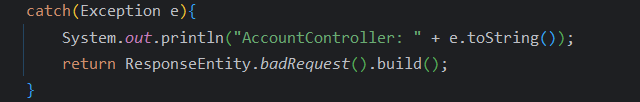
\includegraphics[width=12cm]{images/duplicate.png}}
    \caption[Duplicate Code Section]{Duplicate Code in den catch-Blöcken}
    \label{fig:dc}
\end{figure}

\subsection*{}

Long Method

Complex method

Long Parameter List

Schlechte Fehlermeldungen


%4 Code-Smells nennen und begründen
\section{Refactoring}
\subsection{Magic-Numbers}
Um die zahlreichen \q{Magic-Numbers} im Programmcode entfernen zu können, wurde die Klasse \q{Constants} implementiert. Diese \q{verwaltet} alle Magic-Numbers an einem Ort. Um konstante Werte zu verwenden, müssen andere Klassen diese aus der Constants-Klasse auslesen. Wenn sich in Zukunft eine der Konstanten ändern sollte, muss diese durch die Constants-Klasse nur noch an einer Stelle im Code geändert werden.\\
\url{https://github.com/NI-R0/DH-Software-Engineering-II/commit/d79ca697187f4f855cff56c85f8742fa97d70cda#diff-14e3846dce3ed0f79fab55a1ea9cbdc1b8b56ce2a1080f76df4a5e5b3a3328a0},\\
\url{https://github.com/NI-R0/DH-Software-Engineering-II/commit/d8304e549c5f34f15c279b92706822649fd49f1c#diff-14e3846dce3ed0f79fab55a1ea9cbdc1b8b56ce2a1080f76df4a5e5b3a3328a0}

\subsection{\href{https://refactoring.guru/remove-setting-method}{Setter-Methoden}}
Ein potenzielles Refactoring-Thema, welches zu diesem Zeitpunkt noch nicht verbessert wurde, sind die Setter-Methoden in verschiedenen Klassen (bspw. den Domain-Objekten). Setter-Methoden verletzen das Prinzip der Datenkapselung, wodurch sie theoretisch ermöglichen, Attribute von (Domain-)Objekten auf falsche Werte zu setzen. Anstelle von Setter-Methoden können beispielsweise spezifischere Methoden verwendet werden, die die Parameter auf ihre Korrektheit prüfen, bevor sie das entsprechende Attribut ändern.



% https://refactoring.guru/refactoring/techniques
% https://refactoring.guru/replace-parameter-with-method-call
% https://refactoring.guru/remove-setting-method -> Extra methoden/Factory
% https://refactoring.guru/replace-constructor-with-factory-method -> Factory method
% https://refactoring.guru/consolidate-conditional-expression